\documentclass[12pt,letterpaper]{article}

\usepackage[T1]{fontenc}
\usepackage[margin=1in,headheight=1.5em]{geometry}
\usepackage{enumitem}
\usepackage{fancyhdr}
\usepackage{lastpage}
\usepackage{float}
\usepackage{tabu}
\usepackage{booktabs}
\usepackage{graphicx}
\usepackage{lmodern}

\begin{document}

\renewcommand\headrule{}

\pagestyle{fancy}
\fancyhf{}
\lfoot{COMP 3004}
\rfoot{\thepage/\pageref{LastPage}}
\cfoot{Requirements Analysis Document}

% CUSTOM COMMANDS
\newcommand{\teamname}{Code First, Think Later}
\newcommand{\personone}{Kevin Hua}
\newcommand{\persontwo}{Hendrik Knoetze}
\newcommand{\personthree}{Juhandr\'e Knoetze}
\newcommand{\ccindent}{\hspace{1.5em}\hangindent=1.5em}

%% USE-CASE COMMANDS
\newcounter{usecasenum}
\renewcommand{\theusecasenum}{UC-\ifnum\value{usecasenum}<10 0\fi\arabic{usecasenum}}
\newcommand{\newusecase}[1]{\refstepcounter{usecasenum}\label{#1}\expandafter\newcommand\csname #1\endcsname{\ref{#1}}}

\newusecase{participateinprojects}
\newusecase{manageprojects}
\newusecase{createnewproject}
\newusecase{launchppid}
\newusecase{viewppidresults}
\newusecase{viewppidsummary}
\newusecase{viewppiddetails}
\newusecase{editproject}
\newusecase{editprojectdetails}
\newusecase{editteamsize}
\newusecase{editprojectname}
\newusecase{addstudent}
\newusecase{removestudent}
\newusecase{joinproject}
\newusecase{leaveproject}
\newusecase{editprofile}
\newusecase{editpersonalvalues}
\newusecase{editdesiredvalues}
\newusecase{saveerror}
\newusecase{openerror}
\newusecase{readerror}
\newusecase{writeerror}
\newusecase{closeerror}
\newusecase{invalidinputerror}
\newusecase{illegalminerror}
\newusecase{illegalmaxerror}
\newusecase{projectexistserror}
\newusecase{invalidstudenterror}
\newusecase{insufficientstudentserror}
\newusecase{invalidprojecterror}
%% END USE-CASE COMMANDS
% END CUSTOM COMMANDS

% TABLE STYLING
\everyrow{\hline}
\tabulinesep=0.5em
\setlength\extrarowheight{0.5em}
% END TABLE STYLING

\thispagestyle{empty}

\begin{center}
	CARLETON UNIVERSITY
\end{center}

\vfill

\begin{center}
	{\fontsize{55pt}{55pt}\selectfont cuPID}
	\vspace{0.5em}\rule{\textwidth}{0.5pt}
	Requirements Analysis Document
\end{center}

\vspace{5em}

\begin{center}
	\textbf{Team [\teamname{}]}\\
	\personone{}\\
	\persontwo{}\\
	\personthree{}
\end{center}

\vfill

\begin{center}
	Submitted to:\\
	Dr. Christine Laurendeau\\
	COMP 3004: Object Oriented Software Engineering\\
	School of Computer Science\\
	Carleton University
\end{center}

\vspace{2em}

\begin{center}
	\today
\end{center}

\newpage{}

\tableofcontents{}

\renewcommand{\listfigurename}{Figures}
\listoffigures

\renewcommand{\listtablename}{Tables}
\listoftables

\newpage{}

\section{Introduction}

\begin{center}
    -- project --
\end{center}

\begin{center}
	\Huge [cuPID]
\end{center}

\begin{center}
    \rule{0.85\textwidth}{0.5pt}
\end{center}

\subsection{Purpose of System}

Team projects are typically assigned in University courses in order to develop and foster
good teamwork related skills, which are crucial in most future endeavours, notably 
prospective employment. Unfortunately, the task of separating students into balanced 
and compatible teams has always been a nigh impossible feat - hardly a year passes that doesn't
boast at least a single team brimming with  contention. There just seems to be too many
nuances that are involved in building a perfect team for professors to account for, often leading
to random or pseudo-random assignment of teams. Another possibility that professors might employ
would be to allow the students themselves to form their teams. Regrettably, this option also
leads to much strife - students tend to select friends or acquaintances as partners. While this
solution might seem good, it is sadly the case that good friends often make bad project partners. 
There is also the case that many students have not made friends or acquaintances yet that they 
could ask to be their partners, thus leaving them to form a team with others in their situation.

Both current options leave much to be desired. Our firm, [\teamname{}], has been hired
to design a system that would provide a better solution to this long-standing issue. Thus, the purpose of
our system is to separate students into teams with others of similar personality and skills, eliminating 
the frequent torment associated with ill-matched teams.

\subsection{Overview of Document}

This report provides an overview of the design decisions we made for the cuPID project, including 
use cases, object models, and dynamic models. The goal of this document is to clearly impart our vision of this
program to Dr. Christine Laurendeau, our esteemed employer. In furtherance to this goal, we have painstakingly 
organized our report to maximize both basic legibility and traceability. Before delving into the more complex details 
of our proposed system, we have included a general overview of the elements we wish to incorporate, as well as 
some details with regards to our unique and innovative algorithm.

Following the short synopsis, you will find, the requested requirements, cleanly organized into separate functional 
and non-functional tables. Note that each requirement is assigned a unique but informative identifier - all future references
to this particular requirement will cite its corresponding code. The purpose of the system is, again, to ensure that the
reading of this document is as simple and pleasant an experience as possible. 

Directly after the requirements, we have the various system models. We have chosen to separate them into three
primary categories: the use cases, the objects, and the dynamic models. The goal of this separation scheme is to
stagger the introduction of different components such that the reader does not feel bombarded. Thus, you will 
first see the various possible scenarios and how the system will flow with regards to these scenarios. Subsequently, 
the various objects will be introduced and described in detail. Finally, we will delve into the more detailed sequence 
diagrams that will build on information from the prior sections. This section will handle such things as timings and
the flows for the various possible states of the system.

\vspace{1em}

\noindent Best regards,

\vspace{1em}

\textbf{Team [\teamname{}]}

\newpage{}

\section{Proposed System}

\subsection{Overview}


\subsection{Functional Requirements}

\begin{table}[H]
	\caption{Functional Requirements}
	\vspace{1em}
	\begin{tabu} to \textwidth {>{\bf}lX}
		F-01 & Students must be able to add themselves to any number of projects. \\
		F-02 & Students must be able to remove themselves from a project they are currently part of. \\
		F-03 & Students must be able to edit their Project Partner Profile. \\
		\ccindent{}F-03-01 & \ccindent{}Students must be able to modify the values representing their own qualifications. \\
		\ccindent{}F-03-02 & \ccindent{}Students must be able to modify the values representing what qualifications they
		desire in potential partners (what they prioritize, for example). \\
		F-04 & Students must be able to view their Project Partner Profile. \\
		F-05 & Administrators must be able to create new projects. \\
		F-06 & Administrators must be able to edit existing projects. \\
		\ccindent{}F-06-01 & \ccindent{}Administrators must be able to modify the team size parameter for individual projects. \\
		\ccindent{}F-06-02 & \ccindent{}Administrators must be able to add a student to a selected project. \\
		\ccindent{}F-06-03 & \ccindent{}Administrators must be able to remove a student from a selected project. \\
		\ccindent{}F-06-04 & \ccindent{}Administrators must be able to modify the project name parameter for individual projects.\\
		F-07 & Administrators must be able to launch the PPID for a specific project. \\
		F-08 & Administrators must be able to view the summary results of the last-run PPID. \\
		F-09 & Administrators must be able to view the detailed results of the last-run PPID. \\
	\end{tabu}
\end{table}

\subsection{Non-Functional Requirements}

\begin{table}[H]
	\caption{Non-Functional Requirements}
	\vspace{1em}
	\begin{tabu} to \textwidth {>{\bf}l >{\it}l X}
		NF-01 & Usability & Default keyboard shortcuts must be provided for all users. \\
		NF-02 & Usability & The option to customize the key bindings for default keyboard shortcuts must be available for all users.\\
		NF-03 & Usability & All error messages must be descriptive and suggest appropriate solutions.\\
		NF-04 & Implementation & The software must be written in the C++ language. \\
		NF-05 & Implementation & The software must use the Qt framework for creating the graphical user interface (G.U.I.). \\
		NF-06 & Implementation & The software must run in Linux environment. \\
		NF-07 & Performance & The PPID will take no longer than 5 seconds to finish running. \\
		NF-08 & Reliability & Saved data will remain uncorrupted at least 95\% of the time. \\
		NF-09 & Reliability & Saved information must be backed up. \\
		NF-10 & Supportability & The system must be extensible to a client/server architecture. \\
		NF-11 & Legal & Users must accept a Terms of Service agreement in order to use the software.\\
		NF-12 & Interface & \\
		NF-13 & Operations & A forum should be provided for users to report any bugs they may encounter. \\
		NF-14 & Packaging & The software will be available to download as a standalone executable. \\
	\end{tabu}
\end{table}

\subsection{System Models}

\subsubsection{Use Case Model}



\begin{figure}[H]
	\centering{}
	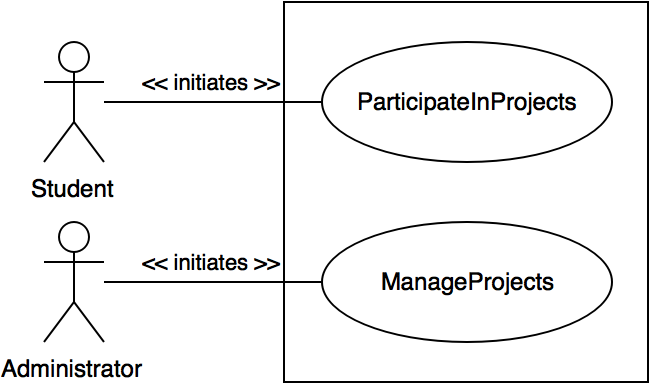
\includegraphics[scale=0.4]{imgs/high-level-use-case-diagram.png}
	\caption{High-level Use Case Diagram}
\end{figure}

\begin{table}[H]
	\caption{High-Level Use Case Descriptions}
	\vspace{1em}
	\begin{tabu} to \textwidth {l >{\bf}l X}
		\participateinprojects{} & ParticipateInProjects & The student accesses and can modify their own profile details 
		(includes project participation details)\\
		\manageprojects{} & ManageProjects & The Administrator manages current project as well as having the option to 
		create a new instance of a project (includes manipulating student participation and access to the PPID and its results). \\
	\end{tabu}
\end{table}

\begin{figure}[H]
	\centering{}
	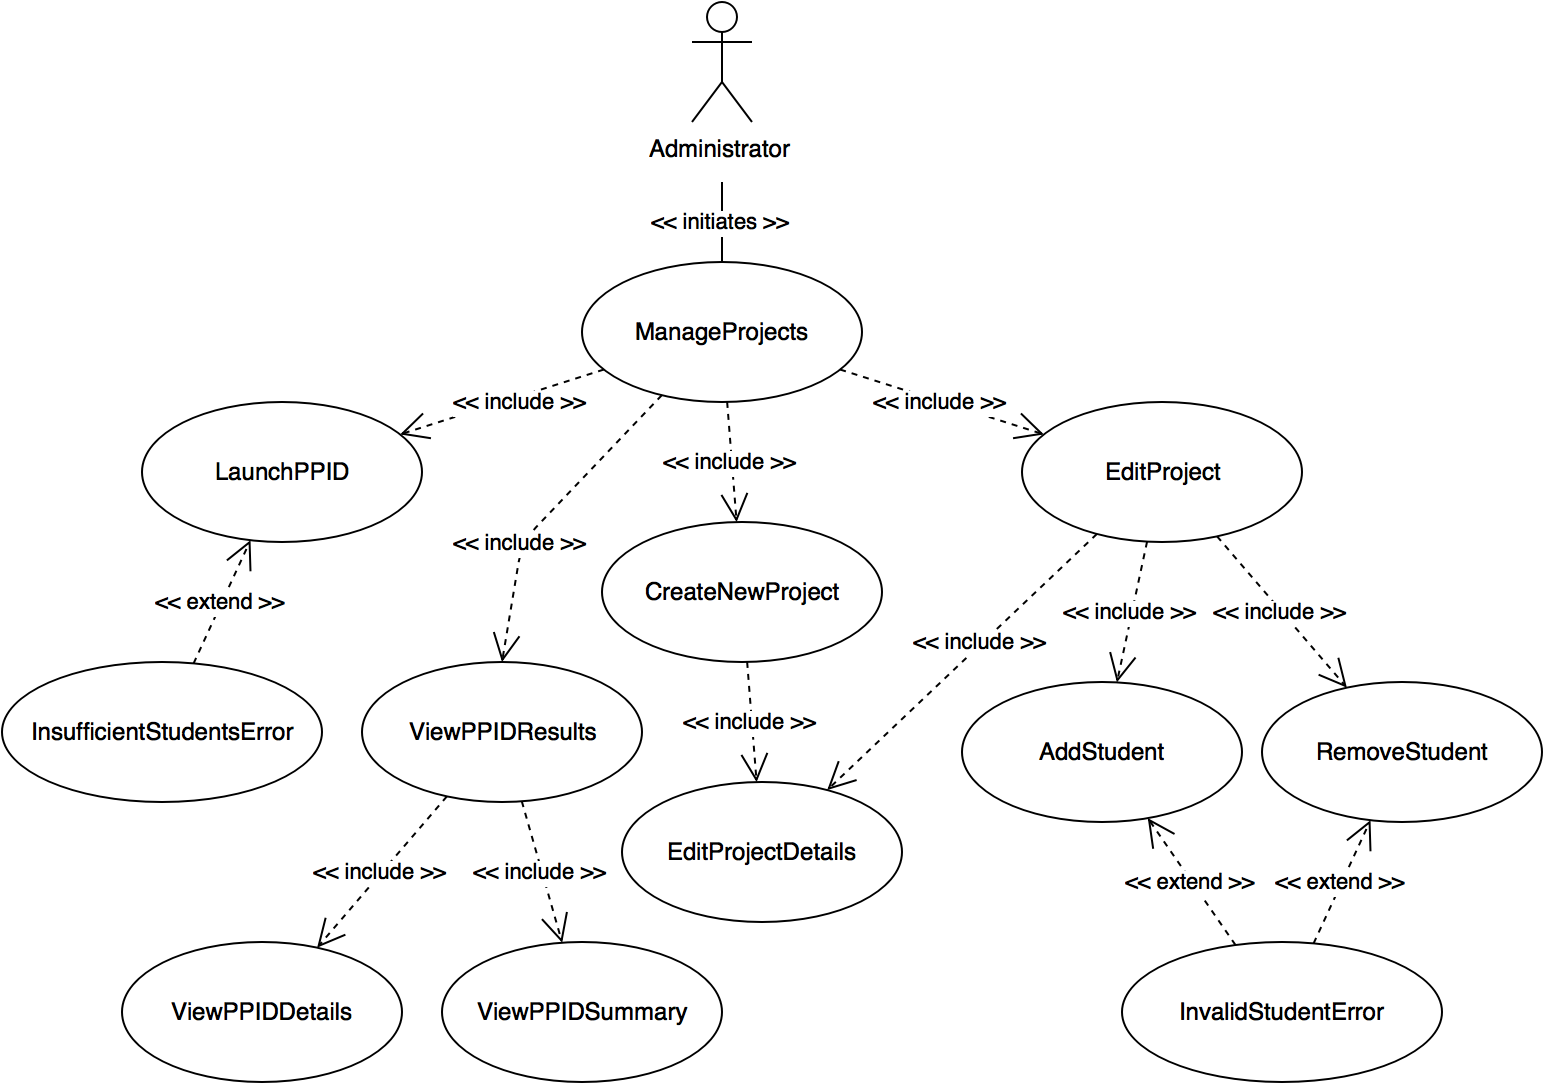
\includegraphics[scale=0.26]{imgs/detailed-administrator-use-case-diagram.png}
	\caption{Detailed Administrator Use Case Diagram}
\end{figure}

\begin{figure}[H]
	\centering{}
	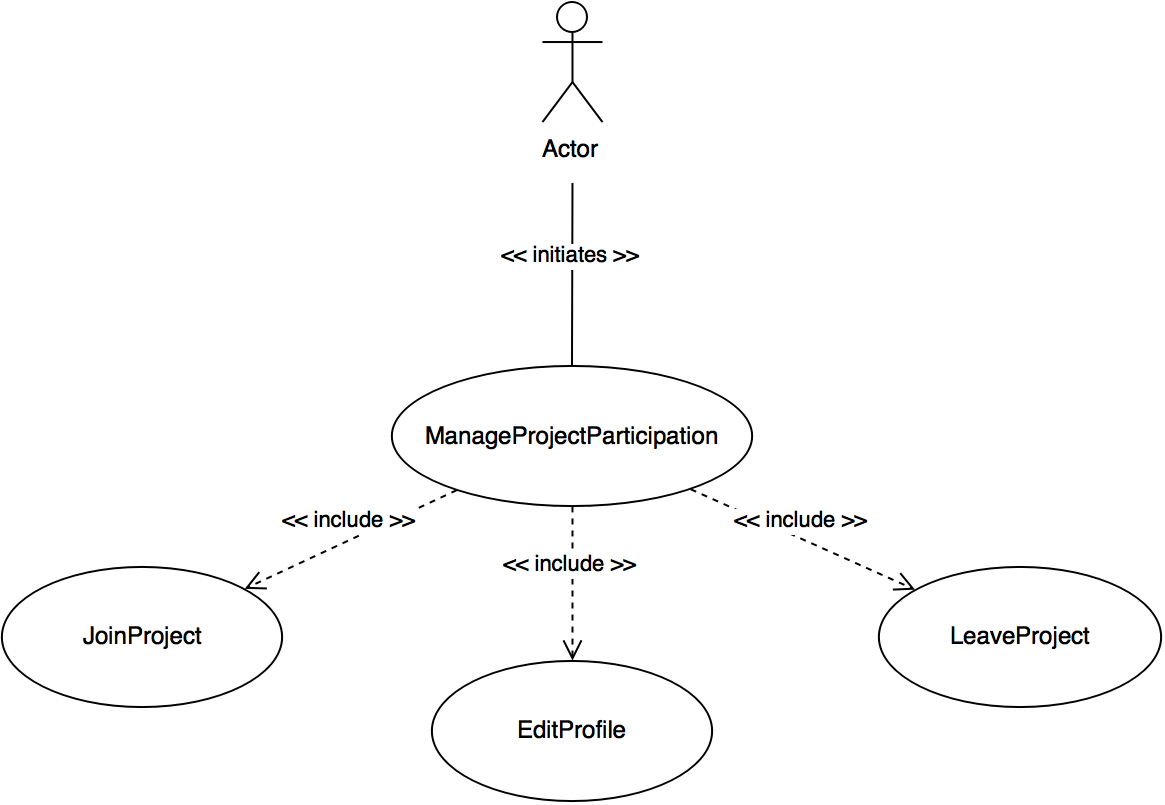
\includegraphics[scale=0.3]{imgs/detailed-student-use-case-diagram.png}
	\caption{Detailed Student Use Case Diagram}
\end{figure}

\begin{figure}[H]
	\centering{}
	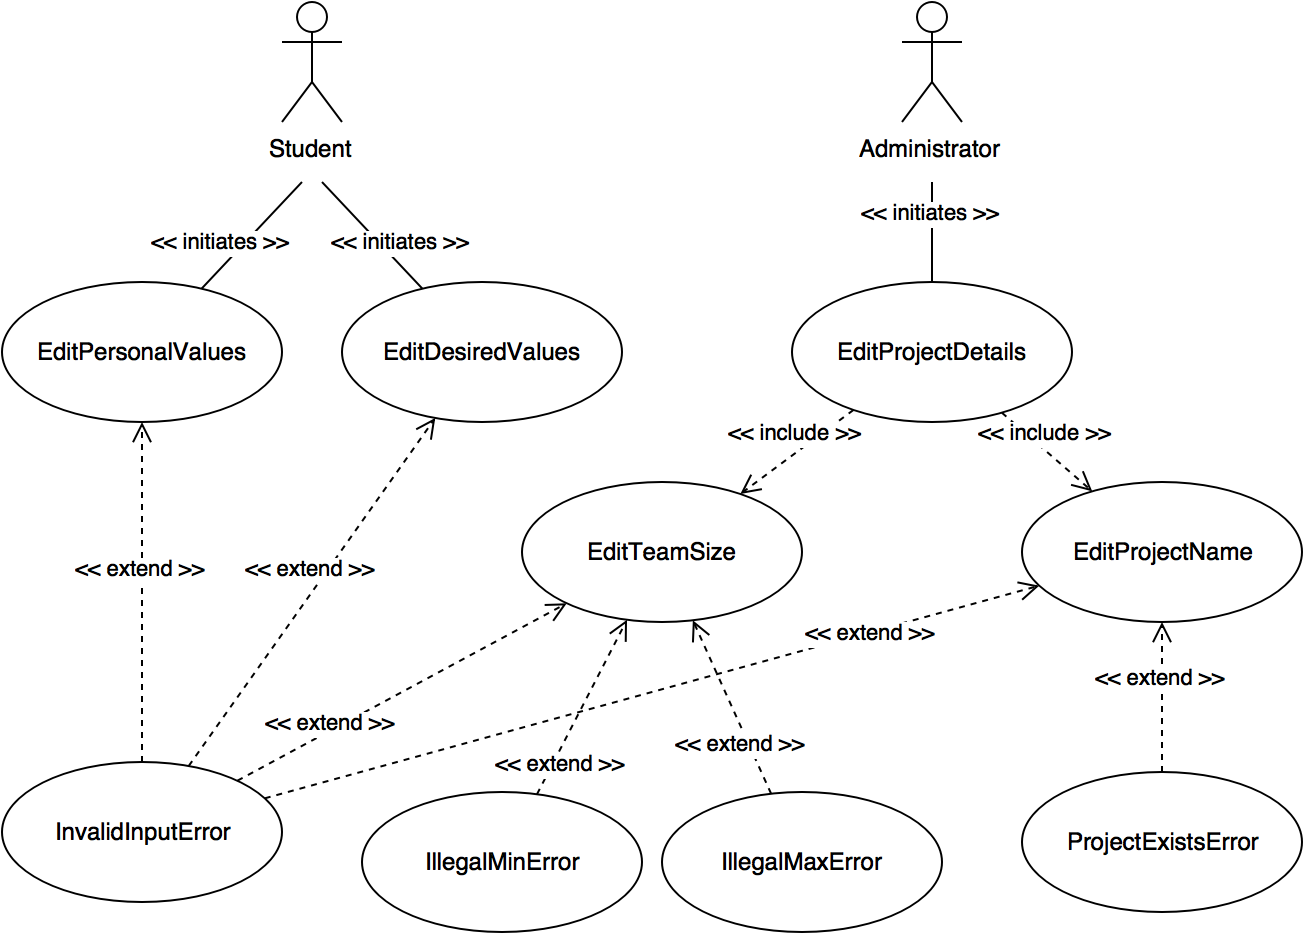
\includegraphics[scale=0.3]{imgs/detailed-user-input-use-case-diagram.png}
	\caption{Detailed User Input Use Case Diagram}
\end{figure}

\begin{table}[H]
	\caption{Detailed Use Case Descriptions - Administrators}
	\vspace{1em}
	\begin{tabu} to \textwidth {l >{\bf}l X}
		\createnewproject{} & CreateNewProject & The Administrator creates a new instance of a project.\\
		\launchppid{} & LaunchPPID & The Administrator runs the PPID for a specified project.\\
		\viewppidresults{} & ViewPPIDResults & The Administrator views the results of the PPID for a project. \\
		\viewppidsummary{} & ViewPPIDSummary & The Administrator views a summary of the groups that are created. \\
		\viewppiddetails{} & ViewPPIDDetails & The Administrator views a detailed analysis of the grouping decisions. \\
		\editproject{} & EditProject & The Administrator modifies an aspect of the project (includes student participation 
		and project parameters).\\
		\editprojectdetails{} & EditProjectDetails & The Administrator modifies the parameters of a specified project.\\
		\editteamsize{} & EditTeamSize & The Administrator sets the minimum and maximum team sizes to be used by the PPID. \\
		\editprojectname{} & EditProjectName & The Administrator sets the name of the project. \\
		\addstudent{} & AddStudent & The Administrator adds a Student to the current project.\\
		\removestudent{} & RemoveStudent & The Administrator removes a Student from the current project.\\
	\end{tabu}
\end{table}

\begin{table}[H]
	\caption{Detailed Use Case Descriptions - Students}
	\vspace{1em}
	\begin{tabu} to \textwidth {l >{\bf}l X}
		\joinproject{} & JoinProject & The student adds themselves to an existing project.\\
		\leaveproject{} & LeaveProject & The student removes themselves from an existing project.\\
		\editprofile{} & EditProfile & The student modifies the parameters of their profile (includes EditPersonalValues and EditDesiredValues).\\
		\editpersonalvalues{} & EditPersonalValues & The student modifies the personal details in his profile (what they have to offer). \\
		\editdesiredvalues{} & EditDesiredValues & The student modifies the desired details in his profile (what they are looking for in 
		potential team members). \\
	\end{tabu}
\end{table}

\begin{table}[H]
	\caption{Detailed Use Case Descriptions - Error Cases}
	\vspace{1em}
	\begin{tabu} to \textwidth {l >{\bf}l X}
		\saveerror{} & SaveError & There was an error during saving (generalizes WriteError, ReadError, OpenError, CloseError). 
		The system reports the specific error to the user and aborts the operation.\\
		\openerror{} & OpenError & The system reports that the selected file could not be opened.\\
		\readerror{} & ReadError & The system reports that the selected file could not be read.\\
		\writeerror{} & WriteError & The system reports that the selected file could not be written to.\\
		\closeerror{} & CloseError & The system reports that the selected file could not be closed.\\
		\invalidinputerror{} & InvalidInputError & The system reports that the given value is invalid.\\
		\illegalminerror{} & IllegalMinError & The system reports that the given minimum team size is illegal.\\
		\illegalmaxerror{} & IllegalMaxError & The system reports that the given maximum team size is illegal.\\
		\projectexistserror{} & ProjectExistsError & The system reports that a project with the given name already exists.\\
		\invalidstudenterror{} & InvalidStudentError & The system reports that an invalid student, be it no student or a non-existent student, was selected to carry out the operation.\\
		\insufficientstudentserror{} & InsufficientStudentsError & The system reports that there are not enough students registered in project to
		 run the PPID.\\
        \invalidprojecterror{} & InvalidProjectError & The system reports that an invalid project, be it no project or a non-existent project, was selected to carry out the operation.\\
	\end{tabu}
\end{table}

\begin{center}
	\begin{tabu} to \textwidth {>{\it}l X}
		\toprule
		Use Case Identifier & \participateinprojects{} \\
		Name & {\bf ParticipateInProjects} \\
		Participating Actors & Initiated by Student \\

		Flow of Events & 
	    \begin{enumerate}[topsep=-1em]
		    \item[1.] The Student begins the cuPID process.
			\begin{enumerate}
				\item[2.] The Student is presented with a menu from the system. Options of: joining a project, leaving a project, or editing their profile for a project.
				\item[3.] If the Student chooses to edit their profile, the system brings up a menu of profile elements that may be modified. The Student may choose to edit their personal details (include use case \textbf{EditPersonalValues}) or to edit their desired partner values (include use case \textbf{EditDesiredValues}).
				\item[4.] If the Student chooses to join a project, the system presents a list of projects to join (include use case \textbf{JoinProject}).
				\item[5.] If the Student chooses to leave a project, the system presents a list of their joined projects to leave (include use case \textbf{LeaveProject}).
			\end{enumerate}
		\end{enumerate} \\

		Entry Conditions & \\

		Exit Conditions & \\ % KEVIN_QUESTION Do we need an exit condition?

		Quality Requirements &
		\begin{itemize}[topsep=-1em]
			\item The user must be operating cuPID as a Student.
		\end{itemize} \\

		Traceability & F-01, F-02, F-03, F-04\\

		\toprule
	\end{tabu}
\end{center}

\begin{center}
    \begin{tabu} to \textwidth {>{\it}l X}
        \toprule
		Use Case Identifier & \manageprojects{} \\
		Name & {\bf ManageProjects} \\
        Participating Actors & Initiated by Administrator \\
		Flow of Events & 
	    \begin{enumerate}[topsep=-1em]
		    \item[1.] The Administrator begins the cuPID process.
			\begin{enumerate}
				\item[2.] The Administrator is presented with a menu from the system. It has the options of: creating a new project, editing a project, launching the PPID, viewing PPID results.
				\item[3.] If the Administrator chooses to create a new project, the system brings up a menu for creating a new project (include use case \textbf{CreateNewProject}).
				\item[4.] If the Administrator chooses to edit a project, the system brings up a list of projects to edit (include use case \textbf{EditProject}).
				\item[5.] If the Administrator chooses to launch the PPID, the system brings up a list of projects (include use case \textbf{LaunchPPID}).
				\item[6.] If the Administrator chooses to view PPID results, the systems brings up a list of projects with PPID results (include use case \textbf{ViewPPIDResults}).
			\end{enumerate}
		\end{enumerate} \\

		Entry Conditions & \\

		Exit Conditions & \\

		Quality Requirements &
		\begin{itemize}[topsep=-1em]
		    \item The user must be operating cuPID as an Administrator. 
        \end{itemize} \\

		Traceability & F-05, F-06, F-07, F-08, F-09\\
        \toprule
    \end{tabu}
\end{center}

\begin{center}
	\begin{tabu} to \textwidth {>{\it}l X}
		\toprule
		Use Case Identifier & \createnewproject{} \\
		Name & {\bf CreateNewProject} \\
		Participating Actors & Initiated by Administrator \\
		Flow of Events & 
	    \begin{enumerate}[topsep=-1em]
		    \item lots of stuff lots of stuff lots of stuff lots of stuff lots of stuff lots of stuff lots of stuff lots of stuff lots of stuff lots of stuff
		    \item other stuff lots of stuff lots of stuff lots of stuff lots of stuff lots of stuff lots of stuff lots of stuff
		\end{enumerate} \\

		Entry Conditions &
		\begin{itemize}[topsep=-1em]
		    \item lots of stuff lots of stuff lots of stuff lots of stuff lots of stuff lots of stuff lots of stuff lots of stuff lots of stuff lots of stuff
		    \item other stuff lots of stuff lots of stuff lots of stuff lots of stuff lots of stuff lots of stuff lots of stuff
        \end{itemize} \\

		Exit Conditions &
		\begin{itemize}[topsep=-1em]
		    \item lots of stuff lots of stuff lots of stuff lots of stuff lots of stuff lots of stuff lots of stuff lots of stuff lots of stuff lots of stuff
		    \item other stuff lots of stuff lots of stuff lots of stuff lots of stuff lots of stuff lots of stuff lots of stuff
        \end{itemize} \\

		Quality Requirements &
		\begin{itemize}[topsep=-1em]
		    \item lots of stuff lots of stuff lots of stuff lots of stuff lots of stuff lots of stuff lots of stuff lots of stuff lots of stuff lots of stuff
		    \item other stuff lots of stuff lots of stuff lots of stuff lots of stuff lots of stuff lots of stuff lots of stuff
        \end{itemize} \\

		Traceability & F-05 \\
		\toprule
	\end{tabu}
\end{center}

\begin{center}
	\begin{tabu} to \textwidth {>{\it}l X}
		\toprule
		Use Case Identifier & \launchppid{} \\
		Name & {\bf LaunchPPID} \\
		Participating Actors & Initiated by Administrator \\
		Flow of Events & 
	    \begin{enumerate}[topsep=-1em]
		    \item lots of stuff lots of stuff lots of stuff lots of stuff lots of stuff lots of stuff lots of stuff lots of stuff lots of stuff lots of stuff
		    \item other stuff lots of stuff lots of stuff lots of stuff lots of stuff lots of stuff lots of stuff lots of stuff
		\end{enumerate} \\

		Entry Conditions &
		\begin{itemize}[topsep=-1em]
		    \item lots of stuff lots of stuff lots of stuff lots of stuff lots of stuff lots of stuff lots of stuff lots of stuff lots of stuff lots of stuff
		    \item other stuff lots of stuff lots of stuff lots of stuff lots of stuff lots of stuff lots of stuff lots of stuff
        \end{itemize} \\

		Exit Conditions &
		\begin{itemize}[topsep=-1em]
		    \item lots of stuff lots of stuff lots of stuff lots of stuff lots of stuff lots of stuff lots of stuff lots of stuff lots of stuff lots of stuff
		    \item other stuff lots of stuff lots of stuff lots of stuff lots of stuff lots of stuff lots of stuff lots of stuff
        \end{itemize} \\

		Quality Requirements &
		\begin{itemize}[topsep=-1em]
		    \item lots of stuff lots of stuff lots of stuff lots of stuff lots of stuff lots of stuff lots of stuff lots of stuff lots of stuff lots of stuff
		    \item other stuff lots of stuff lots of stuff lots of stuff lots of stuff lots of stuff lots of stuff lots of stuff
        \end{itemize} \\

		Traceability & F-07 \\
		\toprule
	\end{tabu}
\end{center}

\begin{center}
	\begin{tabu} to \textwidth {>{\it}l X}
		\toprule
		Use Case Identifier & \viewppidresults{} \\
		Name & {\bf ViewPPIDResults} \\
		Participating Actors & Initiated by Administrator \\
		Flow of Events & 
	    \begin{enumerate}[topsep=-1em]
		    \item lots of stuff lots of stuff lots of stuff lots of stuff lots of stuff lots of stuff lots of stuff lots of stuff lots of stuff lots of stuff
		    \item other stuff lots of stuff lots of stuff lots of stuff lots of stuff lots of stuff lots of stuff lots of stuff
		\end{enumerate} \\

		Entry Conditions &
		\begin{itemize}[topsep=-1em]
		    \item lots of stuff lots of stuff lots of stuff lots of stuff lots of stuff lots of stuff lots of stuff lots of stuff lots of stuff lots of stuff
		    \item other stuff lots of stuff lots of stuff lots of stuff lots of stuff lots of stuff lots of stuff lots of stuff
        \end{itemize} \\

		Exit Conditions &
		\begin{itemize}[topsep=-1em]
		    \item lots of stuff lots of stuff lots of stuff lots of stuff lots of stuff lots of stuff lots of stuff lots of stuff lots of stuff lots of stuff
		    \item other stuff lots of stuff lots of stuff lots of stuff lots of stuff lots of stuff lots of stuff lots of stuff
        \end{itemize} \\

		Quality Requirements &
		\begin{itemize}[topsep=-1em]
		    \item lots of stuff lots of stuff lots of stuff lots of stuff lots of stuff lots of stuff lots of stuff lots of stuff lots of stuff lots of stuff
		    \item other stuff lots of stuff lots of stuff lots of stuff lots of stuff lots of stuff lots of stuff lots of stuff
        \end{itemize} \\

		Traceability & F-08, F-09 \\
		\toprule
	\end{tabu}
\end{center}

\begin{center}
	\begin{tabu} to \textwidth {>{\it}l X}
		\toprule
		Use Case Identifier & \viewppidsummary{} \\
		Name & {\bf ViewPPIDSummary} \\
		Participating Actors & Initiated by Administrator \\
		Flow of Events & 
	    \begin{enumerate}[topsep=-1em]
		    \item lots of stuff lots of stuff lots of stuff lots of stuff lots of stuff lots of stuff lots of stuff lots of stuff lots of stuff lots of stuff
		    \item other stuff lots of stuff lots of stuff lots of stuff lots of stuff lots of stuff lots of stuff lots of stuff
		\end{enumerate} \\

		Entry Conditions &
		\begin{itemize}[topsep=-1em]
		    \item lots of stuff lots of stuff lots of stuff lots of stuff lots of stuff lots of stuff lots of stuff lots of stuff lots of stuff lots of stuff
		    \item other stuff lots of stuff lots of stuff lots of stuff lots of stuff lots of stuff lots of stuff lots of stuff
        \end{itemize} \\

		Exit Conditions &
		\begin{itemize}[topsep=-1em]
		    \item lots of stuff lots of stuff lots of stuff lots of stuff lots of stuff lots of stuff lots of stuff lots of stuff lots of stuff lots of stuff
		    \item other stuff lots of stuff lots of stuff lots of stuff lots of stuff lots of stuff lots of stuff lots of stuff
        \end{itemize} \\

		Quality Requirements &
		\begin{itemize}[topsep=-1em]
		    \item lots of stuff lots of stuff lots of stuff lots of stuff lots of stuff lots of stuff lots of stuff lots of stuff lots of stuff lots of stuff
		    \item other stuff lots of stuff lots of stuff lots of stuff lots of stuff lots of stuff lots of stuff lots of stuff
        \end{itemize} \\

		Traceability & F-08 \\
		\toprule
	\end{tabu}
\end{center}

\begin{center}
	\begin{tabu} to \textwidth {>{\it}l X}
		\toprule
		Use Case Identifier & \viewppiddetails{} \\
		Name & {\bf ViewPPIDDetails} \\
		Participating Actors & Initiated by Administrator \\
		Flow of Events & 
	    \begin{enumerate}[topsep=-1em]
		    \item lots of stuff lots of stuff lots of stuff lots of stuff lots of stuff lots of stuff lots of stuff lots of stuff lots of stuff lots of stuff
		    \item other stuff lots of stuff lots of stuff lots of stuff lots of stuff lots of stuff lots of stuff lots of stuff
		\end{enumerate} \\

		Entry Conditions &
		\begin{itemize}[topsep=-1em]
		    \item lots of stuff lots of stuff lots of stuff lots of stuff lots of stuff lots of stuff lots of stuff lots of stuff lots of stuff lots of stuff
		    \item other stuff lots of stuff lots of stuff lots of stuff lots of stuff lots of stuff lots of stuff lots of stuff
        \end{itemize} \\

		Exit Conditions &
		\begin{itemize}[topsep=-1em]
		    \item lots of stuff lots of stuff lots of stuff lots of stuff lots of stuff lots of stuff lots of stuff lots of stuff lots of stuff lots of stuff
		    \item other stuff lots of stuff lots of stuff lots of stuff lots of stuff lots of stuff lots of stuff lots of stuff
        \end{itemize} \\

		Quality Requirements &
		\begin{itemize}[topsep=-1em]
		    \item lots of stuff lots of stuff lots of stuff lots of stuff lots of stuff lots of stuff lots of stuff lots of stuff lots of stuff lots of stuff
		    \item other stuff lots of stuff lots of stuff lots of stuff lots of stuff lots of stuff lots of stuff lots of stuff
        \end{itemize} \\

		Traceability & F-09 \\
		\toprule
	\end{tabu}
\end{center}

\begin{center}
	\begin{tabu} to \textwidth {>{\it}l X}
		\toprule
		Use Case Identifier & \editproject{} \\
		Name & {\bf EditProject} \\
		Participating Actors & Initiated by Administrator \\
		Flow of Events & 
	    \begin{enumerate}[topsep=-1em]
		    \item lots of stuff lots of stuff lots of stuff lots of stuff lots of stuff lots of stuff lots of stuff lots of stuff lots of stuff lots of stuff
		    \item other stuff lots of stuff lots of stuff lots of stuff lots of stuff lots of stuff lots of stuff lots of stuff
		\end{enumerate} \\

		Entry Conditions &
		\begin{itemize}[topsep=-1em]
		    \item lots of stuff lots of stuff lots of stuff lots of stuff lots of stuff lots of stuff lots of stuff lots of stuff lots of stuff lots of stuff
		    \item other stuff lots of stuff lots of stuff lots of stuff lots of stuff lots of stuff lots of stuff lots of stuff
        \end{itemize} \\

		Exit Conditions &
		\begin{itemize}[topsep=-1em]
		    \item lots of stuff lots of stuff lots of stuff lots of stuff lots of stuff lots of stuff lots of stuff lots of stuff lots of stuff lots of stuff
		    \item other stuff lots of stuff lots of stuff lots of stuff lots of stuff lots of stuff lots of stuff lots of stuff
        \end{itemize} \\

		Quality Requirements &
		\begin{itemize}[topsep=-1em]
		    \item lots of stuff lots of stuff lots of stuff lots of stuff lots of stuff lots of stuff lots of stuff lots of stuff lots of stuff lots of stuff
		    \item other stuff lots of stuff lots of stuff lots of stuff lots of stuff lots of stuff lots of stuff lots of stuff
        \end{itemize} \\

		Traceability & F-06 \\
		\toprule
	\end{tabu}
\end{center}

\begin{center}
	\begin{tabu} to \textwidth {>{\it}l X}
		\toprule
		Use Case Identifier & \editprojectdetails{} \\
		Name & {\bf EditProjectDetails} \\
		Participating Actors & Initiated by Administrator \\
		Flow of Events & 
	    \begin{enumerate}[topsep=-1em]
		    \item lots of stuff lots of stuff lots of stuff lots of stuff lots of stuff lots of stuff lots of stuff lots of stuff lots of stuff lots of stuff
		    \item other stuff lots of stuff lots of stuff lots of stuff lots of stuff lots of stuff lots of stuff lots of stuff
		\end{enumerate} \\

		Entry Conditions &
		\begin{itemize}[topsep=-1em]
		    \item lots of stuff lots of stuff lots of stuff lots of stuff lots of stuff lots of stuff lots of stuff lots of stuff lots of stuff lots of stuff
		    \item other stuff lots of stuff lots of stuff lots of stuff lots of stuff lots of stuff lots of stuff lots of stuff
        \end{itemize} \\

		Exit Conditions &
		\begin{itemize}[topsep=-1em]
		    \item lots of stuff lots of stuff lots of stuff lots of stuff lots of stuff lots of stuff lots of stuff lots of stuff lots of stuff lots of stuff
		    \item other stuff lots of stuff lots of stuff lots of stuff lots of stuff lots of stuff lots of stuff lots of stuff
        \end{itemize} \\

		Quality Requirements &
		\begin{itemize}[topsep=-1em]
		    \item lots of stuff lots of stuff lots of stuff lots of stuff lots of stuff lots of stuff lots of stuff lots of stuff lots of stuff lots of stuff
		    \item other stuff lots of stuff lots of stuff lots of stuff lots of stuff lots of stuff lots of stuff lots of stuff
        \end{itemize} \\

		Traceability & F-05, F-06, F-06-01, F-06-04 \\
		\toprule
	\end{tabu}
\end{center}

\begin{center}
	\begin{tabu} to \textwidth {>{\it}l X}
		\toprule
		Use Case Identifier & \editteamsize{} \\
		Name & {\bf EditTeamSize} \\
		Participating Actors & Initiated by Administrator \\
		Flow of Events & 
	    \begin{enumerate}[topsep=-1em]
		    \item lots of stuff lots of stuff lots of stuff lots of stuff lots of stuff lots of stuff lots of stuff lots of stuff lots of stuff lots of stuff
		    \item other stuff lots of stuff lots of stuff lots of stuff lots of stuff lots of stuff lots of stuff lots of stuff
		\end{enumerate} \\

		Entry Conditions &
		\begin{itemize}[topsep=-1em]
		    \item lots of stuff lots of stuff lots of stuff lots of stuff lots of stuff lots of stuff lots of stuff lots of stuff lots of stuff lots of stuff
		    \item other stuff lots of stuff lots of stuff lots of stuff lots of stuff lots of stuff lots of stuff lots of stuff
        \end{itemize} \\

		Exit Conditions &
		\begin{itemize}[topsep=-1em]
		    \item lots of stuff lots of stuff lots of stuff lots of stuff lots of stuff lots of stuff lots of stuff lots of stuff lots of stuff lots of stuff
		    \item other stuff lots of stuff lots of stuff lots of stuff lots of stuff lots of stuff lots of stuff lots of stuff
        \end{itemize} \\

		Quality Requirements &
		\begin{itemize}[topsep=-1em]
		    \item lots of stuff lots of stuff lots of stuff lots of stuff lots of stuff lots of stuff lots of stuff lots of stuff lots of stuff lots of stuff
		    \item other stuff lots of stuff lots of stuff lots of stuff lots of stuff lots of stuff lots of stuff lots of stuff
        \end{itemize} \\

		Traceability & F-06-01 \\
		\toprule
	\end{tabu}
\end{center}

\begin{center}
	\begin{tabu} to \textwidth {>{\it}l X}
		\toprule
		Use Case Identifier & \editprojectname{} \\
		Name & {\bf EditProjectName} \\
		Participating Actors & Initiated by Administrator \\
		Flow of Events & 
	    \begin{enumerate}[topsep=-1em]
		    \item lots of stuff lots of stuff lots of stuff lots of stuff lots of stuff lots of stuff lots of stuff lots of stuff lots of stuff lots of stuff
		    \item other stuff lots of stuff lots of stuff lots of stuff lots of stuff lots of stuff lots of stuff lots of stuff
		\end{enumerate} \\

		Entry Conditions &
		\begin{itemize}[topsep=-1em]
		    \item lots of stuff lots of stuff lots of stuff lots of stuff lots of stuff lots of stuff lots of stuff lots of stuff lots of stuff lots of stuff
		    \item other stuff lots of stuff lots of stuff lots of stuff lots of stuff lots of stuff lots of stuff lots of stuff
        \end{itemize} \\

		Exit Conditions &
		\begin{itemize}[topsep=-1em]
		    \item lots of stuff lots of stuff lots of stuff lots of stuff lots of stuff lots of stuff lots of stuff lots of stuff lots of stuff lots of stuff
		    \item other stuff lots of stuff lots of stuff lots of stuff lots of stuff lots of stuff lots of stuff lots of stuff
        \end{itemize} \\

		Quality Requirements &
		\begin{itemize}[topsep=-1em]
		    \item lots of stuff lots of stuff lots of stuff lots of stuff lots of stuff lots of stuff lots of stuff lots of stuff lots of stuff lots of stuff
		    \item other stuff lots of stuff lots of stuff lots of stuff lots of stuff lots of stuff lots of stuff lots of stuff
        \end{itemize} \\

		Traceability & F-06-04 \\
		\toprule
	\end{tabu}
\end{center}

\begin{center}
	\begin{tabu} to \textwidth {>{\it}l X}
		\toprule
		Use Case Identifier & \addstudent{} \\
		Name & {\bf AddStudent} \\
		Participating Actors & Initiated by Administrator \\
		Flow of Events & 
	    \begin{enumerate}[topsep=-1em]
		    \item lots of stuff lots of stuff lots of stuff lots of stuff lots of stuff lots of stuff lots of stuff lots of stuff lots of stuff lots of stuff
		    \item other stuff lots of stuff lots of stuff lots of stuff lots of stuff lots of stuff lots of stuff lots of stuff
		\end{enumerate} \\

		Entry Conditions &
		\begin{itemize}[topsep=-1em]
		    \item lots of stuff lots of stuff lots of stuff lots of stuff lots of stuff lots of stuff lots of stuff lots of stuff lots of stuff lots of stuff
		    \item other stuff lots of stuff lots of stuff lots of stuff lots of stuff lots of stuff lots of stuff lots of stuff
        \end{itemize} \\

		Exit Conditions &
		\begin{itemize}[topsep=-1em]
		    \item lots of stuff lots of stuff lots of stuff lots of stuff lots of stuff lots of stuff lots of stuff lots of stuff lots of stuff lots of stuff
		    \item other stuff lots of stuff lots of stuff lots of stuff lots of stuff lots of stuff lots of stuff lots of stuff
        \end{itemize} \\

		Quality Requirements &
		\begin{itemize}[topsep=-1em]
		    \item lots of stuff lots of stuff lots of stuff lots of stuff lots of stuff lots of stuff lots of stuff lots of stuff lots of stuff lots of stuff
		    \item other stuff lots of stuff lots of stuff lots of stuff lots of stuff lots of stuff lots of stuff lots of stuff
        \end{itemize} \\

		Traceability & F-06-02 \\
		\toprule
	\end{tabu}
\end{center}

\begin{center}
	\begin{tabu} to \textwidth {>{\it}l X}
		\toprule
		Use Case Identifier & \removestudent{} \\
		Name & {\bf RemoveStudent} \\
		Participating Actors & Initiated by Administrator \\
		Flow of Events & 
	    \begin{enumerate}[topsep=-1em]
		    \item lots of stuff lots of stuff lots of stuff lots of stuff lots of stuff lots of stuff lots of stuff lots of stuff lots of stuff lots of stuff
		    \item other stuff lots of stuff lots of stuff lots of stuff lots of stuff lots of stuff lots of stuff lots of stuff
		\end{enumerate} \\

		Entry Conditions &
		\begin{itemize}[topsep=-1em]
		    \item lots of stuff lots of stuff lots of stuff lots of stuff lots of stuff lots of stuff lots of stuff lots of stuff lots of stuff lots of stuff
		    \item other stuff lots of stuff lots of stuff lots of stuff lots of stuff lots of stuff lots of stuff lots of stuff
        \end{itemize} \\

		Exit Conditions &
		\begin{itemize}[topsep=-1em]
		    \item lots of stuff lots of stuff lots of stuff lots of stuff lots of stuff lots of stuff lots of stuff lots of stuff lots of stuff lots of stuff
		    \item other stuff lots of stuff lots of stuff lots of stuff lots of stuff lots of stuff lots of stuff lots of stuff
        \end{itemize} \\

		Quality Requirements &
		\begin{itemize}[topsep=-1em]
		    \item lots of stuff lots of stuff lots of stuff lots of stuff lots of stuff lots of stuff lots of stuff lots of stuff lots of stuff lots of stuff
		    \item other stuff lots of stuff lots of stuff lots of stuff lots of stuff lots of stuff lots of stuff lots of stuff
        \end{itemize} \\

		Traceability & F-06-03 \\
		\toprule
	\end{tabu}
\end{center}

\begin{center}
	\begin{tabu} to \textwidth {>{\it}l X}
		\toprule
		Use Case Identifier & \joinproject{} \\
		Name & {\bf JoinProject} \\
		Participating Actors & Initiated by Student \\
		Flow of Events & 
	    \begin{enumerate}[topsep=-1em]
		    \item lots of stuff lots of stuff lots of stuff lots of stuff lots of stuff lots of stuff lots of stuff lots of stuff lots of stuff lots of stuff
		    \item other stuff lots of stuff lots of stuff lots of stuff lots of stuff lots of stuff lots of stuff lots of stuff
		\end{enumerate} \\

		Entry Conditions &
		\begin{itemize}[topsep=-1em]
		    \item lots of stuff lots of stuff lots of stuff lots of stuff lots of stuff lots of stuff lots of stuff lots of stuff lots of stuff lots of stuff
		    \item other stuff lots of stuff lots of stuff lots of stuff lots of stuff lots of stuff lots of stuff lots of stuff
        \end{itemize} \\

		Exit Conditions &
		\begin{itemize}[topsep=-1em]
		    \item lots of stuff lots of stuff lots of stuff lots of stuff lots of stuff lots of stuff lots of stuff lots of stuff lots of stuff lots of stuff
		    \item other stuff lots of stuff lots of stuff lots of stuff lots of stuff lots of stuff lots of stuff lots of stuff
        \end{itemize} \\

		Quality Requirements &
		\begin{itemize}[topsep=-1em]
		    \item lots of stuff lots of stuff lots of stuff lots of stuff lots of stuff lots of stuff lots of stuff lots of stuff lots of stuff lots of stuff
		    \item other stuff lots of stuff lots of stuff lots of stuff lots of stuff lots of stuff lots of stuff lots of stuff
        \end{itemize} \\

		Traceability & NF-03 \\
		\toprule
	\end{tabu}
\end{center}

\begin{center}
	\begin{tabu} to \textwidth {>{\it}l X}
		\toprule
		Use Case Identifier & \leaveproject{} \\
		Name & {\bf LeaveProject} \\
		Participating Actors & Initiated by Student \\
		Flow of Events & 
	    \begin{enumerate}[topsep=-1em]
		    \item lots of stuff lots of stuff lots of stuff lots of stuff lots of stuff lots of stuff lots of stuff lots of stuff lots of stuff lots of stuff
		    \item other stuff lots of stuff lots of stuff lots of stuff lots of stuff lots of stuff lots of stuff lots of stuff
		\end{enumerate} \\

		Entry Conditions &
		\begin{itemize}[topsep=-1em]
		    \item lots of stuff lots of stuff lots of stuff lots of stuff lots of stuff lots of stuff lots of stuff lots of stuff lots of stuff lots of stuff
		    \item other stuff lots of stuff lots of stuff lots of stuff lots of stuff lots of stuff lots of stuff lots of stuff
        \end{itemize} \\

		Exit Conditions &
		\begin{itemize}[topsep=-1em]
		    \item lots of stuff lots of stuff lots of stuff lots of stuff lots of stuff lots of stuff lots of stuff lots of stuff lots of stuff lots of stuff
		    \item other stuff lots of stuff lots of stuff lots of stuff lots of stuff lots of stuff lots of stuff lots of stuff
        \end{itemize} \\

		Quality Requirements &
		\begin{itemize}[topsep=-1em]
		    \item lots of stuff lots of stuff lots of stuff lots of stuff lots of stuff lots of stuff lots of stuff lots of stuff lots of stuff lots of stuff
		    \item other stuff lots of stuff lots of stuff lots of stuff lots of stuff lots of stuff lots of stuff lots of stuff
        \end{itemize} \\

		Traceability & NF-03 \\
		\toprule
	\end{tabu}
\end{center}

\begin{center}
	\begin{tabu} to \textwidth {>{\it}l X}
		\toprule
		Use Case Identifier & \editprofile{} \\
		Name & {\bf EditProfile} \\
		Participating Actors & Initiated by Student \\
		Flow of Events & 
	    \begin{enumerate}[topsep=-1em]
		    \item lots of stuff lots of stuff lots of stuff lots of stuff lots of stuff lots of stuff lots of stuff lots of stuff lots of stuff lots of stuff
		    \item other stuff lots of stuff lots of stuff lots of stuff lots of stuff lots of stuff lots of stuff lots of stuff
		\end{enumerate} \\

		Entry Conditions &
		\begin{itemize}[topsep=-1em]
		    \item lots of stuff lots of stuff lots of stuff lots of stuff lots of stuff lots of stuff lots of stuff lots of stuff lots of stuff lots of stuff
		    \item other stuff lots of stuff lots of stuff lots of stuff lots of stuff lots of stuff lots of stuff lots of stuff
        \end{itemize} \\

		Exit Conditions &
		\begin{itemize}[topsep=-1em]
		    \item lots of stuff lots of stuff lots of stuff lots of stuff lots of stuff lots of stuff lots of stuff lots of stuff lots of stuff lots of stuff
		    \item other stuff lots of stuff lots of stuff lots of stuff lots of stuff lots of stuff lots of stuff lots of stuff
        \end{itemize} \\

		Quality Requirements &
		\begin{itemize}[topsep=-1em]
		    \item lots of stuff lots of stuff lots of stuff lots of stuff lots of stuff lots of stuff lots of stuff lots of stuff lots of stuff lots of stuff
		    \item other stuff lots of stuff lots of stuff lots of stuff lots of stuff lots of stuff lots of stuff lots of stuff
        \end{itemize} \\

		Traceability & NF-03 \\
		\toprule
	\end{tabu}
\end{center}

\begin{center}
	\begin{tabu} to \textwidth {>{\it}l X}
		\toprule
		Use Case Identifier & \editpersonalvalues{} \\
		Name & {\bf EditPersonalValues} \\
		Participating Actors & Initiated by Student \\
		Flow of Events & 
	    \begin{enumerate}[topsep=-1em]
		    \item lots of stuff lots of stuff lots of stuff lots of stuff lots of stuff lots of stuff lots of stuff lots of stuff lots of stuff lots of stuff
		    \item other stuff lots of stuff lots of stuff lots of stuff lots of stuff lots of stuff lots of stuff lots of stuff
		\end{enumerate} \\

		Entry Conditions &
		\begin{itemize}[topsep=-1em]
		    \item lots of stuff lots of stuff lots of stuff lots of stuff lots of stuff lots of stuff lots of stuff lots of stuff lots of stuff lots of stuff
		    \item other stuff lots of stuff lots of stuff lots of stuff lots of stuff lots of stuff lots of stuff lots of stuff
        \end{itemize} \\

		Exit Conditions &
		\begin{itemize}[topsep=-1em]
		    \item lots of stuff lots of stuff lots of stuff lots of stuff lots of stuff lots of stuff lots of stuff lots of stuff lots of stuff lots of stuff
		    \item other stuff lots of stuff lots of stuff lots of stuff lots of stuff lots of stuff lots of stuff lots of stuff
        \end{itemize} \\

		Quality Requirements &
		\begin{itemize}[topsep=-1em]
		    \item lots of stuff lots of stuff lots of stuff lots of stuff lots of stuff lots of stuff lots of stuff lots of stuff lots of stuff lots of stuff
		    \item other stuff lots of stuff lots of stuff lots of stuff lots of stuff lots of stuff lots of stuff lots of stuff
        \end{itemize} \\

		Traceability & NF-03 \\
		\toprule
	\end{tabu}
\end{center}

\begin{center}
	\begin{tabu} to \textwidth {>{\it}l X}
		\toprule
		Use Case Identifier & \editdesiredvalues{} \\
		Name & {\bf EditDesiredValues} \\
		Participating Actors & Initiated by Student \\
		Flow of Events & 
	    \begin{enumerate}[topsep=-1em]
		    \item lots of stuff lots of stuff lots of stuff lots of stuff lots of stuff lots of stuff lots of stuff lots of stuff lots of stuff lots of stuff
		    \item other stuff lots of stuff lots of stuff lots of stuff lots of stuff lots of stuff lots of stuff lots of stuff
		\end{enumerate} \\

		Entry Conditions &
		\begin{itemize}[topsep=-1em]
		    \item lots of stuff lots of stuff lots of stuff lots of stuff lots of stuff lots of stuff lots of stuff lots of stuff lots of stuff lots of stuff
		    \item other stuff lots of stuff lots of stuff lots of stuff lots of stuff lots of stuff lots of stuff lots of stuff
        \end{itemize} \\

		Exit Conditions &
		\begin{itemize}[topsep=-1em]
		    \item lots of stuff lots of stuff lots of stuff lots of stuff lots of stuff lots of stuff lots of stuff lots of stuff lots of stuff lots of stuff
		    \item other stuff lots of stuff lots of stuff lots of stuff lots of stuff lots of stuff lots of stuff lots of stuff
        \end{itemize} \\

		Quality Requirements &
		\begin{itemize}[topsep=-1em]
		    \item lots of stuff lots of stuff lots of stuff lots of stuff lots of stuff lots of stuff lots of stuff lots of stuff lots of stuff lots of stuff
		    \item other stuff lots of stuff lots of stuff lots of stuff lots of stuff lots of stuff lots of stuff lots of stuff
        \end{itemize} \\

		Traceability & NF-03 \\
		\toprule
	\end{tabu}
\end{center}

\begin{center}
	\begin{tabu} to \textwidth {>{\it}l X}
		\toprule
		Use Case Identifier & \saveerror{} \\
		Name & {\bf SaveError} \\
		Participating Actors & Administrator \\
		Flow of Events & 
	    \begin{enumerate}[topsep=-1em]
		    \item The system notifies the Administrator that an error has occured with regards to the processing of
		    the current file.
		\end{enumerate} \\

		Entry Conditions &
		\begin{itemize}[topsep=-1em]
		    \item A file processing operation failed.
        \end{itemize} \\

		Exit Conditions &
		\begin{itemize}[topsep=-1em]
		    \item The operation is aborted.
        \end{itemize} \\

		Quality Requirements &
		\begin{itemize}[topsep=-1em]
		    \item 
        \end{itemize} \\

		Traceability & NF-03 \\
		\toprule
	\end{tabu}
\end{center}

\begin{center}
	\begin{tabu} to \textwidth {>{\it}l X}
		\toprule
		Use Case Identifier & \openerror{} \\
		Name & {\bf OpenError} \\
		Participating Actors & Administrator \\
		Flow of Events & 
	    \begin{enumerate}[topsep=-1em]
		    \item lots of stuff lots of stuff lots of stuff lots of stuff lots of stuff lots of stuff lots of stuff lots of stuff lots of stuff lots of stuff
		    \item other stuff lots of stuff lots of stuff lots of stuff lots of stuff lots of stuff lots of stuff lots of stuff
		\end{enumerate} \\

		Entry Conditions &
		\begin{itemize}[topsep=-1em]
		    \item lots of stuff lots of stuff lots of stuff lots of stuff lots of stuff lots of stuff lots of stuff lots of stuff lots of stuff lots of stuff
		    \item other stuff lots of stuff lots of stuff lots of stuff lots of stuff lots of stuff lots of stuff lots of stuff
        \end{itemize} \\

		Exit Conditions &
		\begin{itemize}[topsep=-1em]
		    \item lots of stuff lots of stuff lots of stuff lots of stuff lots of stuff lots of stuff lots of stuff lots of stuff lots of stuff lots of stuff
		    \item other stuff lots of stuff lots of stuff lots of stuff lots of stuff lots of stuff lots of stuff lots of stuff
        \end{itemize} \\

		Quality Requirements &
		\begin{itemize}[topsep=-1em]
		    \item lots of stuff lots of stuff lots of stuff lots of stuff lots of stuff lots of stuff lots of stuff lots of stuff lots of stuff lots of stuff
		    \item other stuff lots of stuff lots of stuff lots of stuff lots of stuff lots of stuff lots of stuff lots of stuff
        \end{itemize} \\

		Traceability & NF-03 \\
		\toprule
	\end{tabu}
\end{center}

\begin{center}
	\begin{tabu} to \textwidth {>{\it}l X}
		\toprule
		Use Case Identifier & \readerror{} \\
		Name & {\bf ReadError} \\
		Participating Actors & Administrator \\
		Flow of Events & 
	    \begin{enumerate}[topsep=-1em]
		    \item lots of stuff lots of stuff lots of stuff lots of stuff lots of stuff lots of stuff lots of stuff lots of stuff lots of stuff lots of stuff
		    \item other stuff lots of stuff lots of stuff lots of stuff lots of stuff lots of stuff lots of stuff lots of stuff
		\end{enumerate} \\

		Entry Conditions &
		\begin{itemize}[topsep=-1em]
		    \item lots of stuff lots of stuff lots of stuff lots of stuff lots of stuff lots of stuff lots of stuff lots of stuff lots of stuff lots of stuff
		    \item other stuff lots of stuff lots of stuff lots of stuff lots of stuff lots of stuff lots of stuff lots of stuff
        \end{itemize} \\

		Exit Conditions &
		\begin{itemize}[topsep=-1em]
		    \item lots of stuff lots of stuff lots of stuff lots of stuff lots of stuff lots of stuff lots of stuff lots of stuff lots of stuff lots of stuff
		    \item other stuff lots of stuff lots of stuff lots of stuff lots of stuff lots of stuff lots of stuff lots of stuff
        \end{itemize} \\

		Quality Requirements &
		\begin{itemize}[topsep=-1em]
		    \item lots of stuff lots of stuff lots of stuff lots of stuff lots of stuff lots of stuff lots of stuff lots of stuff lots of stuff lots of stuff
		    \item other stuff lots of stuff lots of stuff lots of stuff lots of stuff lots of stuff lots of stuff lots of stuff
        \end{itemize} \\

		Traceability & NF-03 \\
		\toprule
	\end{tabu}
\end{center}

\begin{center}
	\begin{tabu} to \textwidth {>{\it}l X}
		\toprule
		Use Case Identifier & \writeerror{} \\
		Name & {\bf WriteError} \\
		Participating Actors & Administrator \\
		Flow of Events & 
	    \begin{enumerate}[topsep=-1em]
		    \item lots of stuff lots of stuff lots of stuff lots of stuff lots of stuff lots of stuff lots of stuff lots of stuff lots of stuff lots of stuff
		    \item other stuff lots of stuff lots of stuff lots of stuff lots of stuff lots of stuff lots of stuff lots of stuff
		\end{enumerate} \\

		Entry Conditions &
		\begin{itemize}[topsep=-1em]
		    \item lots of stuff lots of stuff lots of stuff lots of stuff lots of stuff lots of stuff lots of stuff lots of stuff lots of stuff lots of stuff
		    \item other stuff lots of stuff lots of stuff lots of stuff lots of stuff lots of stuff lots of stuff lots of stuff
        \end{itemize} \\

		Exit Conditions &
		\begin{itemize}[topsep=-1em]
		    \item lots of stuff lots of stuff lots of stuff lots of stuff lots of stuff lots of stuff lots of stuff lots of stuff lots of stuff lots of stuff
		    \item other stuff lots of stuff lots of stuff lots of stuff lots of stuff lots of stuff lots of stuff lots of stuff
        \end{itemize} \\

		Quality Requirements &
		\begin{itemize}[topsep=-1em]
		    \item lots of stuff lots of stuff lots of stuff lots of stuff lots of stuff lots of stuff lots of stuff lots of stuff lots of stuff lots of stuff
		    \item other stuff lots of stuff lots of stuff lots of stuff lots of stuff lots of stuff lots of stuff lots of stuff
        \end{itemize} \\

		Traceability & NF-03 \\
		\toprule
	\end{tabu}
\end{center}

\begin{center}
	\begin{tabu} to \textwidth {>{\it}l X}
		\toprule
		Use Case Identifier & \closeerror{} \\
		Name & {\bf CloseError} \\
		Participating Actors & Administrator \\
		Flow of Events & 
	    \begin{enumerate}[topsep=-1em]
		    \item lots of stuff lots of stuff lots of stuff lots of stuff lots of stuff lots of stuff lots of stuff lots of stuff lots of stuff lots of stuff
		    \item other stuff lots of stuff lots of stuff lots of stuff lots of stuff lots of stuff lots of stuff lots of stuff
		\end{enumerate} \\

		Entry Conditions &
		\begin{itemize}[topsep=-1em]
		    \item lots of stuff lots of stuff lots of stuff lots of stuff lots of stuff lots of stuff lots of stuff lots of stuff lots of stuff lots of stuff
		    \item other stuff lots of stuff lots of stuff lots of stuff lots of stuff lots of stuff lots of stuff lots of stuff
        \end{itemize} \\

		Exit Conditions &
		\begin{itemize}[topsep=-1em]
		    \item lots of stuff lots of stuff lots of stuff lots of stuff lots of stuff lots of stuff lots of stuff lots of stuff lots of stuff lots of stuff
		    \item other stuff lots of stuff lots of stuff lots of stuff lots of stuff lots of stuff lots of stuff lots of stuff
        \end{itemize} \\

		Quality Requirements &
		\begin{itemize}[topsep=-1em]
		    \item lots of stuff lots of stuff lots of stuff lots of stuff lots of stuff lots of stuff lots of stuff lots of stuff lots of stuff lots of stuff
		    \item other stuff lots of stuff lots of stuff lots of stuff lots of stuff lots of stuff lots of stuff lots of stuff
        \end{itemize} \\

		Traceability & NF-03 \\
		\toprule
	\end{tabu}
\end{center}

\begin{center}
	\begin{tabu} to \textwidth {>{\it}l X}
		\toprule
		Use Case Identifier & \invalidinputerror{} \\
		Name & {\bf InvalidInputError} \\
		Participating Actors & Administrator, Student \\
		Flow of Events & 
	    \begin{enumerate}[topsep=-1em]
		    \item lots of stuff lots of stuff lots of stuff lots of stuff lots of stuff lots of stuff lots of stuff lots of stuff lots of stuff lots of stuff
		    \item other stuff lots of stuff lots of stuff lots of stuff lots of stuff lots of stuff lots of stuff lots of stuff
		\end{enumerate} \\

		Entry Conditions &
		\begin{itemize}[topsep=-1em]
		    \item lots of stuff lots of stuff lots of stuff lots of stuff lots of stuff lots of stuff lots of stuff lots of stuff lots of stuff lots of stuff
		    \item other stuff lots of stuff lots of stuff lots of stuff lots of stuff lots of stuff lots of stuff lots of stuff
        \end{itemize} \\

		Exit Conditions &
		\begin{itemize}[topsep=-1em]
		    \item lots of stuff lots of stuff lots of stuff lots of stuff lots of stuff lots of stuff lots of stuff lots of stuff lots of stuff lots of stuff
		    \item other stuff lots of stuff lots of stuff lots of stuff lots of stuff lots of stuff lots of stuff lots of stuff
        \end{itemize} \\

		Quality Requirements &
		\begin{itemize}[topsep=-1em]
		    \item lots of stuff lots of stuff lots of stuff lots of stuff lots of stuff lots of stuff lots of stuff lots of stuff lots of stuff lots of stuff
		    \item other stuff lots of stuff lots of stuff lots of stuff lots of stuff lots of stuff lots of stuff lots of stuff
        \end{itemize} \\

		Traceability & NF-03 \\
		\toprule
	\end{tabu}
\end{center}

\begin{center}
	\begin{tabu} to \textwidth {>{\it}l X}
		\toprule
		Use Case Identifier & \illegalminerror{} \\
		Name & {\bf IllegalMinError} \\
		Participating Actors & Administrator \\
		Flow of Events & 
	    \begin{enumerate}[topsep=-1em]
		    \item lots of stuff lots of stuff lots of stuff lots of stuff lots of stuff lots of stuff lots of stuff lots of stuff lots of stuff lots of stuff
		    \item other stuff lots of stuff lots of stuff lots of stuff lots of stuff lots of stuff lots of stuff lots of stuff
		\end{enumerate} \\

		Entry Conditions &
		\begin{itemize}[topsep=-1em]
		    \item lots of stuff lots of stuff lots of stuff lots of stuff lots of stuff lots of stuff lots of stuff lots of stuff lots of stuff lots of stuff
		    \item other stuff lots of stuff lots of stuff lots of stuff lots of stuff lots of stuff lots of stuff lots of stuff
        \end{itemize} \\

		Exit Conditions &
		\begin{itemize}[topsep=-1em]
		    \item lots of stuff lots of stuff lots of stuff lots of stuff lots of stuff lots of stuff lots of stuff lots of stuff lots of stuff lots of stuff
		    \item other stuff lots of stuff lots of stuff lots of stuff lots of stuff lots of stuff lots of stuff lots of stuff
        \end{itemize} \\

		Quality Requirements &
		\begin{itemize}[topsep=-1em]
		    \item lots of stuff lots of stuff lots of stuff lots of stuff lots of stuff lots of stuff lots of stuff lots of stuff lots of stuff lots of stuff
		    \item other stuff lots of stuff lots of stuff lots of stuff lots of stuff lots of stuff lots of stuff lots of stuff
        \end{itemize} \\

		Traceability & NF-03 \\
		\toprule
	\end{tabu}
\end{center}

\begin{center}
	\begin{tabu} to \textwidth {>{\it}l X}
		\toprule
		Use Case Identifier & \illegalmaxerror{} \\
		Name & {\bf IllegalMaxError} \\
		Participating Actors & Administrator \\
		Flow of Events & 
	    \begin{enumerate}[topsep=-1em]
		    \item lots of stuff lots of stuff lots of stuff lots of stuff lots of stuff lots of stuff lots of stuff lots of stuff lots of stuff lots of stuff
		    \item other stuff lots of stuff lots of stuff lots of stuff lots of stuff lots of stuff lots of stuff lots of stuff
		\end{enumerate} \\

		Entry Conditions &
		\begin{itemize}[topsep=-1em]
		    \item lots of stuff lots of stuff lots of stuff lots of stuff lots of stuff lots of stuff lots of stuff lots of stuff lots of stuff lots of stuff
		    \item other stuff lots of stuff lots of stuff lots of stuff lots of stuff lots of stuff lots of stuff lots of stuff
        \end{itemize} \\

		Exit Conditions &
		\begin{itemize}[topsep=-1em]
		    \item lots of stuff lots of stuff lots of stuff lots of stuff lots of stuff lots of stuff lots of stuff lots of stuff lots of stuff lots of stuff
		    \item other stuff lots of stuff lots of stuff lots of stuff lots of stuff lots of stuff lots of stuff lots of stuff
        \end{itemize} \\

		Quality Requirements &
		\begin{itemize}[topsep=-1em]
		    \item lots of stuff lots of stuff lots of stuff lots of stuff lots of stuff lots of stuff lots of stuff lots of stuff lots of stuff lots of stuff
		    \item other stuff lots of stuff lots of stuff lots of stuff lots of stuff lots of stuff lots of stuff lots of stuff
        \end{itemize} \\

		Traceability & NF-03 \\
		\toprule
	\end{tabu}
\end{center}

\begin{center}
	\begin{tabu} to \textwidth {>{\it}l X}
		\toprule
		Use Case Identifier & \projectexistserror{} \\
		Name & {\bf ProjectExistsError} \\
		Participating Actors & Administrator \\
		Flow of Events & 
	    \begin{enumerate}[topsep=-1em]
		    \item lots of stuff lots of stuff lots of stuff lots of stuff lots of stuff lots of stuff lots of stuff lots of stuff lots of stuff lots of stuff
		    \item other stuff lots of stuff lots of stuff lots of stuff lots of stuff lots of stuff lots of stuff lots of stuff
		\end{enumerate} \\

		Entry Conditions &
		\begin{itemize}[topsep=-1em]
		    \item lots of stuff lots of stuff lots of stuff lots of stuff lots of stuff lots of stuff lots of stuff lots of stuff lots of stuff lots of stuff
		    \item other stuff lots of stuff lots of stuff lots of stuff lots of stuff lots of stuff lots of stuff lots of stuff
        \end{itemize} \\

		Exit Conditions &
		\begin{itemize}[topsep=-1em]
		    \item lots of stuff lots of stuff lots of stuff lots of stuff lots of stuff lots of stuff lots of stuff lots of stuff lots of stuff lots of stuff
		    \item other stuff lots of stuff lots of stuff lots of stuff lots of stuff lots of stuff lots of stuff lots of stuff
        \end{itemize} \\

		Quality Requirements &
		\begin{itemize}[topsep=-1em]
		    \item lots of stuff lots of stuff lots of stuff lots of stuff lots of stuff lots of stuff lots of stuff lots of stuff lots of stuff lots of stuff
		    \item other stuff lots of stuff lots of stuff lots of stuff lots of stuff lots of stuff lots of stuff lots of stuff
        \end{itemize} \\

		Traceability & NF-03 \\
		\toprule
	\end{tabu}
\end{center}

\begin{center}
	\begin{tabu} to \textwidth {>{\it}l X}
		\toprule
		Use Case Identifier & \invalidstudenterror{} \\
		Name & {\bf InvalidStudentError} \\
		Participating Actors & Administrator \\
		Flow of Events & 
	    \begin{enumerate}[topsep=-1em]
		    \item lots of stuff lots of stuff lots of stuff lots of stuff lots of stuff lots of stuff lots of stuff lots of stuff lots of stuff lots of stuff
		    \item other stuff lots of stuff lots of stuff lots of stuff lots of stuff lots of stuff lots of stuff lots of stuff
		\end{enumerate} \\

		Entry Conditions &
		\begin{itemize}[topsep=-1em]
		    \item lots of stuff lots of stuff lots of stuff lots of stuff lots of stuff lots of stuff lots of stuff lots of stuff lots of stuff lots of stuff
		    \item other stuff lots of stuff lots of stuff lots of stuff lots of stuff lots of stuff lots of stuff lots of stuff
        \end{itemize} \\

		Exit Conditions &
		\begin{itemize}[topsep=-1em]
		    \item lots of stuff lots of stuff lots of stuff lots of stuff lots of stuff lots of stuff lots of stuff lots of stuff lots of stuff lots of stuff
		    \item other stuff lots of stuff lots of stuff lots of stuff lots of stuff lots of stuff lots of stuff lots of stuff
        \end{itemize} \\

		Quality Requirements &
		\begin{itemize}[topsep=-1em]
		    \item lots of stuff lots of stuff lots of stuff lots of stuff lots of stuff lots of stuff lots of stuff lots of stuff lots of stuff lots of stuff
		    \item other stuff lots of stuff lots of stuff lots of stuff lots of stuff lots of stuff lots of stuff lots of stuff
        \end{itemize} \\

		Traceability & NF-03 \\
		\toprule
	\end{tabu}
\end{center}

\begin{center}
	\begin{tabu} to \textwidth {>{\it}l X}
		\toprule
		Use Case Identifier & \insufficientstudentserror{} \\
		Name & {\bf InsufficientStudentsError} \\
		Participating Actors & Administrator \\
		Flow of Events & 
	    \begin{enumerate}[topsep=-1em]
		    \item lots of stuff lots of stuff lots of stuff lots of stuff lots of stuff lots of stuff lots of stuff lots of stuff lots of stuff lots of stuff
		    \item other stuff lots of stuff lots of stuff lots of stuff lots of stuff lots of stuff lots of stuff lots of stuff
		\end{enumerate} \\

		Entry Conditions &
		\begin{itemize}[topsep=-1em]
		    \item lots of stuff lots of stuff lots of stuff lots of stuff lots of stuff lots of stuff lots of stuff lots of stuff lots of stuff lots of stuff
		    \item other stuff lots of stuff lots of stuff lots of stuff lots of stuff lots of stuff lots of stuff lots of stuff
        \end{itemize} \\

		Exit Conditions &
		\begin{itemize}[topsep=-1em]
		    \item lots of stuff lots of stuff lots of stuff lots of stuff lots of stuff lots of stuff lots of stuff lots of stuff lots of stuff lots of stuff
		    \item other stuff lots of stuff lots of stuff lots of stuff lots of stuff lots of stuff lots of stuff lots of stuff
        \end{itemize} \\

		Quality Requirements &
		\begin{itemize}[topsep=-1em]
		    \item lots of stuff lots of stuff lots of stuff lots of stuff lots of stuff lots of stuff lots of stuff lots of stuff lots of stuff lots of stuff
		    \item other stuff lots of stuff lots of stuff lots of stuff lots of stuff lots of stuff lots of stuff lots of stuff
        \end{itemize} \\

		Traceability & NF-03 \\
		\toprule
	\end{tabu}
\end{center}

\begin{center}
	\begin{tabu} to \textwidth {>{\it}l X}
		\toprule
		Use Case Identifier & \invalidprojecterror{} \\
		Name & {\bf InvalidProjectError} \\
		Participating Actors & Student \\
		Flow of Events & 
	    \begin{enumerate}[topsep=-1em]
		    \item lots of stuff lots of stuff lots of stuff lots of stuff lots of stuff lots of stuff lots of stuff lots of stuff lots of stuff lots of stuff
		    \item other stuff lots of stuff lots of stuff lots of stuff lots of stuff lots of stuff lots of stuff lots of stuff
		\end{enumerate} \\

		Entry Conditions &
		\begin{itemize}[topsep=-1em]
		    \item lots of stuff lots of stuff lots of stuff lots of stuff lots of stuff lots of stuff lots of stuff lots of stuff lots of stuff lots of stuff
		    \item other stuff lots of stuff lots of stuff lots of stuff lots of stuff lots of stuff lots of stuff lots of stuff
        \end{itemize} \\

		Exit Conditions &
		\begin{itemize}[topsep=-1em]
		    \item lots of stuff lots of stuff lots of stuff lots of stuff lots of stuff lots of stuff lots of stuff lots of stuff lots of stuff lots of stuff
		    \item other stuff lots of stuff lots of stuff lots of stuff lots of stuff lots of stuff lots of stuff lots of stuff
        \end{itemize} \\

		Quality Requirements &
		\begin{itemize}[topsep=-1em]
		    \item lots of stuff lots of stuff lots of stuff lots of stuff lots of stuff lots of stuff lots of stuff lots of stuff lots of stuff lots of stuff
		    \item other stuff lots of stuff lots of stuff lots of stuff lots of stuff lots of stuff lots of stuff lots of stuff
        \end{itemize} \\

		Traceability & NF-03 \\
		\toprule
	\end{tabu}
\end{center}

\subsubsection{Object Model}


\subsubsection{Dynamic Model}


\end{document}
